\documentclass[12pt]{article}
\usepackage[a4paper,margin=2cm]{geometry}
\usepackage{fontspec}
\setmainfont{Times New Roman}
\usepackage{graphicx}
\usepackage{tikz}
\usepackage{float}
\usepackage{booktabs}
\usepackage{xcolor}
\usepackage[hidelinks]{hyperref}
\usetikzlibrary{positioning,arrows.meta}
\setlength{\parindent}{0pt}
\setlength{\parskip}{6pt}
\sloppy
\newcommand{\shot}[3]{%
  \begin{figure}[H]\centering
  \includegraphics[width=\textwidth,height=#2,keepaspectratio]{#1}
  \caption{#3}
  \end{figure}}
\title{Source-Code Evidence for the Real-Time AI Governance Audit Pipeline}
\author{Aditya Ranjan \and Arindam Gupta \and Gnanendra Naidu N}
\date{November 2026}

\begin{document}
\maketitle
\thispagestyle{empty}

\begin{abstract}
This document records the implemented pipeline using screenshots generated directly from the repository source files. Each screenshot is tied to a source path and represents the corresponding stage described in the project report. The sequence follows the exact flow: producer adapters, Kafka topics and configuration, Kafka Streams processing, governance rules, risk scoring, PostgreSQL evidence, agent investigation and review, evaluation and recovery, and reporting.
\end{abstract}

\section*{Pipeline represented in the report}
\begin{center}
\resizebox{0.98\textwidth}{!}{%
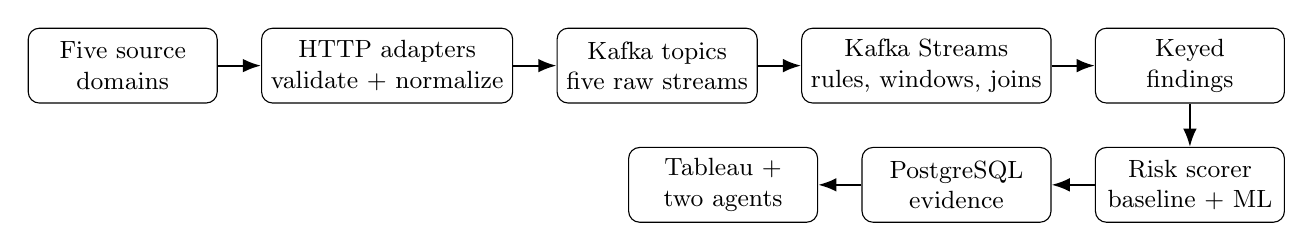
\begin{tikzpicture}[box/.style={draw,rounded corners,align=center,minimum height=0.95cm,minimum width=2.4cm,font=\small},arr/.style={-Latex,thick},node distance=0.55cm]
\node[box] (src) {Five source\\domains};
\node[box,right=of src] (adp) {HTTP adapters\\validate + normalize};
\node[box,right=of adp] (kaf) {Kafka topics\\five raw streams};
\node[box,right=of kaf] (str) {Kafka Streams\\rules, windows, joins};
\node[box,right=of str] (fin) {Keyed\\findings};
\node[box,below=of fin] (risk) {Risk scorer\\baseline + ML};
\node[box,left=of risk] (db) {PostgreSQL\\evidence};
\node[box,left=of db] (out) {Tableau +\\two agents};
\draw[arr] (src)--(adp); \draw[arr] (adp)--(kaf); \draw[arr] (kaf)--(str); \draw[arr] (str)--(fin); \draw[arr] (fin)--(risk); \draw[arr] (risk)--(db); \draw[arr] (db)--(out);
\end{tikzpicture}}
\end{center}

The screenshots are not mock-ups or reconstructed examples. They are rendered views of source excerpts read from the working repository. The source path is printed in each image header so that every implementation claim can be traced to a file.

\clearpage
\section{1. Producer adapters and event normalization}
The pipeline starts with five producer domains: Keycloak identity, Kubernetes audit, Airflow/OpenLineage pipeline activity, model registry activity, and LLM gateway activity. The shared mapper layer converts source-specific payloads into the canonical governance-event contract while retaining source identifiers and evidence metadata.
\shot{01-github-producer-adapter.png}{0.56\textheight}{Actual GitHub source page for the producer adapter mapping layer.}
\shot{02-github-kafka-configuration.png}{0.44\textheight}{Actual GitHub source page for Kafka-compatible broker, topic, and service configuration.}

\clearpage
\section{2. Kafka topics and stream processing}
The normalized events are published to dedicated raw topics. The stream processor consumes those topics using Kafka Streams. The implementation uses event timestamps, state stores, windows, table-table joins, stream-table joins, keyed findings, and JSON serialization. The screenshot below is the actual topology source used to connect those operations.
\shot{03-github-stream-topology.png}{0.68\textheight}{Actual GitHub source page for the Kafka Streams topology, rules, windows, joins, and finding emission.}

\clearpage
\section{3. Governance rule catalogue}
The rule catalogue is configuration-driven. It associates executable controls with severity and governance-framework metadata. Rule identity is preserved in every finding so that a reviewer can connect a result to the exact configured condition.
\shot{04-github-rule-catalogue.png}{0.73\textheight}{Actual GitHub source page for the configured governance rule catalogue.}

\clearpage
\section{4. Risk scoring and durable evidence}
After stream processing, findings are scored and persisted. The risk service keeps the deterministic baseline visible and adds an online Isolation Forest comparison once sufficient history is available. The PostgreSQL sink performs idempotent writes for events, findings, evidence, and scores.
\shot{05-github-risk-scoring.png}{0.55\textheight}{Actual GitHub source page for deterministic baseline and Isolation Forest risk scoring.}
\shot{06-github-postgres-persistence.png}{0.45\textheight}{Actual GitHub source page for durable, idempotent PostgreSQL evidence persistence.}

\clearpage
\section{5. Investigator and Evidence Reviewer agents}
The agents run after durable evidence exists. The Investigator retrieves eligible evidence and writes a structured report. The Evidence Reviewer checks citations and completeness, may request a bounded correction, and can terminate with human review. Neither agent is an infrastructure-remediation authority.
\shot{07-github-investigator-agent.png}{0.56\textheight}{Actual GitHub source page for Amazon Bedrock Investigator report generation.}
\shot{08-github-reviewer-workflow.png}{0.44\textheight}{Actual GitHub source page for Evidence Reviewer validation, bounded revision, and terminal states.}

\clearpage
\section{6. Evaluation and recovery evidence}
The repository evaluation uses labelled source-shaped events and expected findings. The recorded demonstration contains 72 events and 48 expected findings across 16 rules. Baseline, processor-replacement, broker-restart, adapter, consumer-tail, and agent-review checks are kept as repository artefacts.
\shot{09-github-evaluation-results.png}{0.63\textheight}{Actual GitHub source page for recorded evaluation results.}
\shot{10-github-recovery-evaluation.png}{0.43\textheight}{Actual GitHub source page for restart, replay, and resilience verification.}

\clearpage
\section{7. Reporting output}
The final stage exposes durable evidence through reporting views. The dashboard consumes stored findings, risk scores, framework associations, latency observations, and incident details. It is downstream of the detection and persistence path and does not replace the evidence records.
\shot{11-github-reporting-schema.png}{0.53\textheight}{Actual GitHub source page for the reporting schema exposing persisted governance evidence.}
\begin{figure}[H]\centering
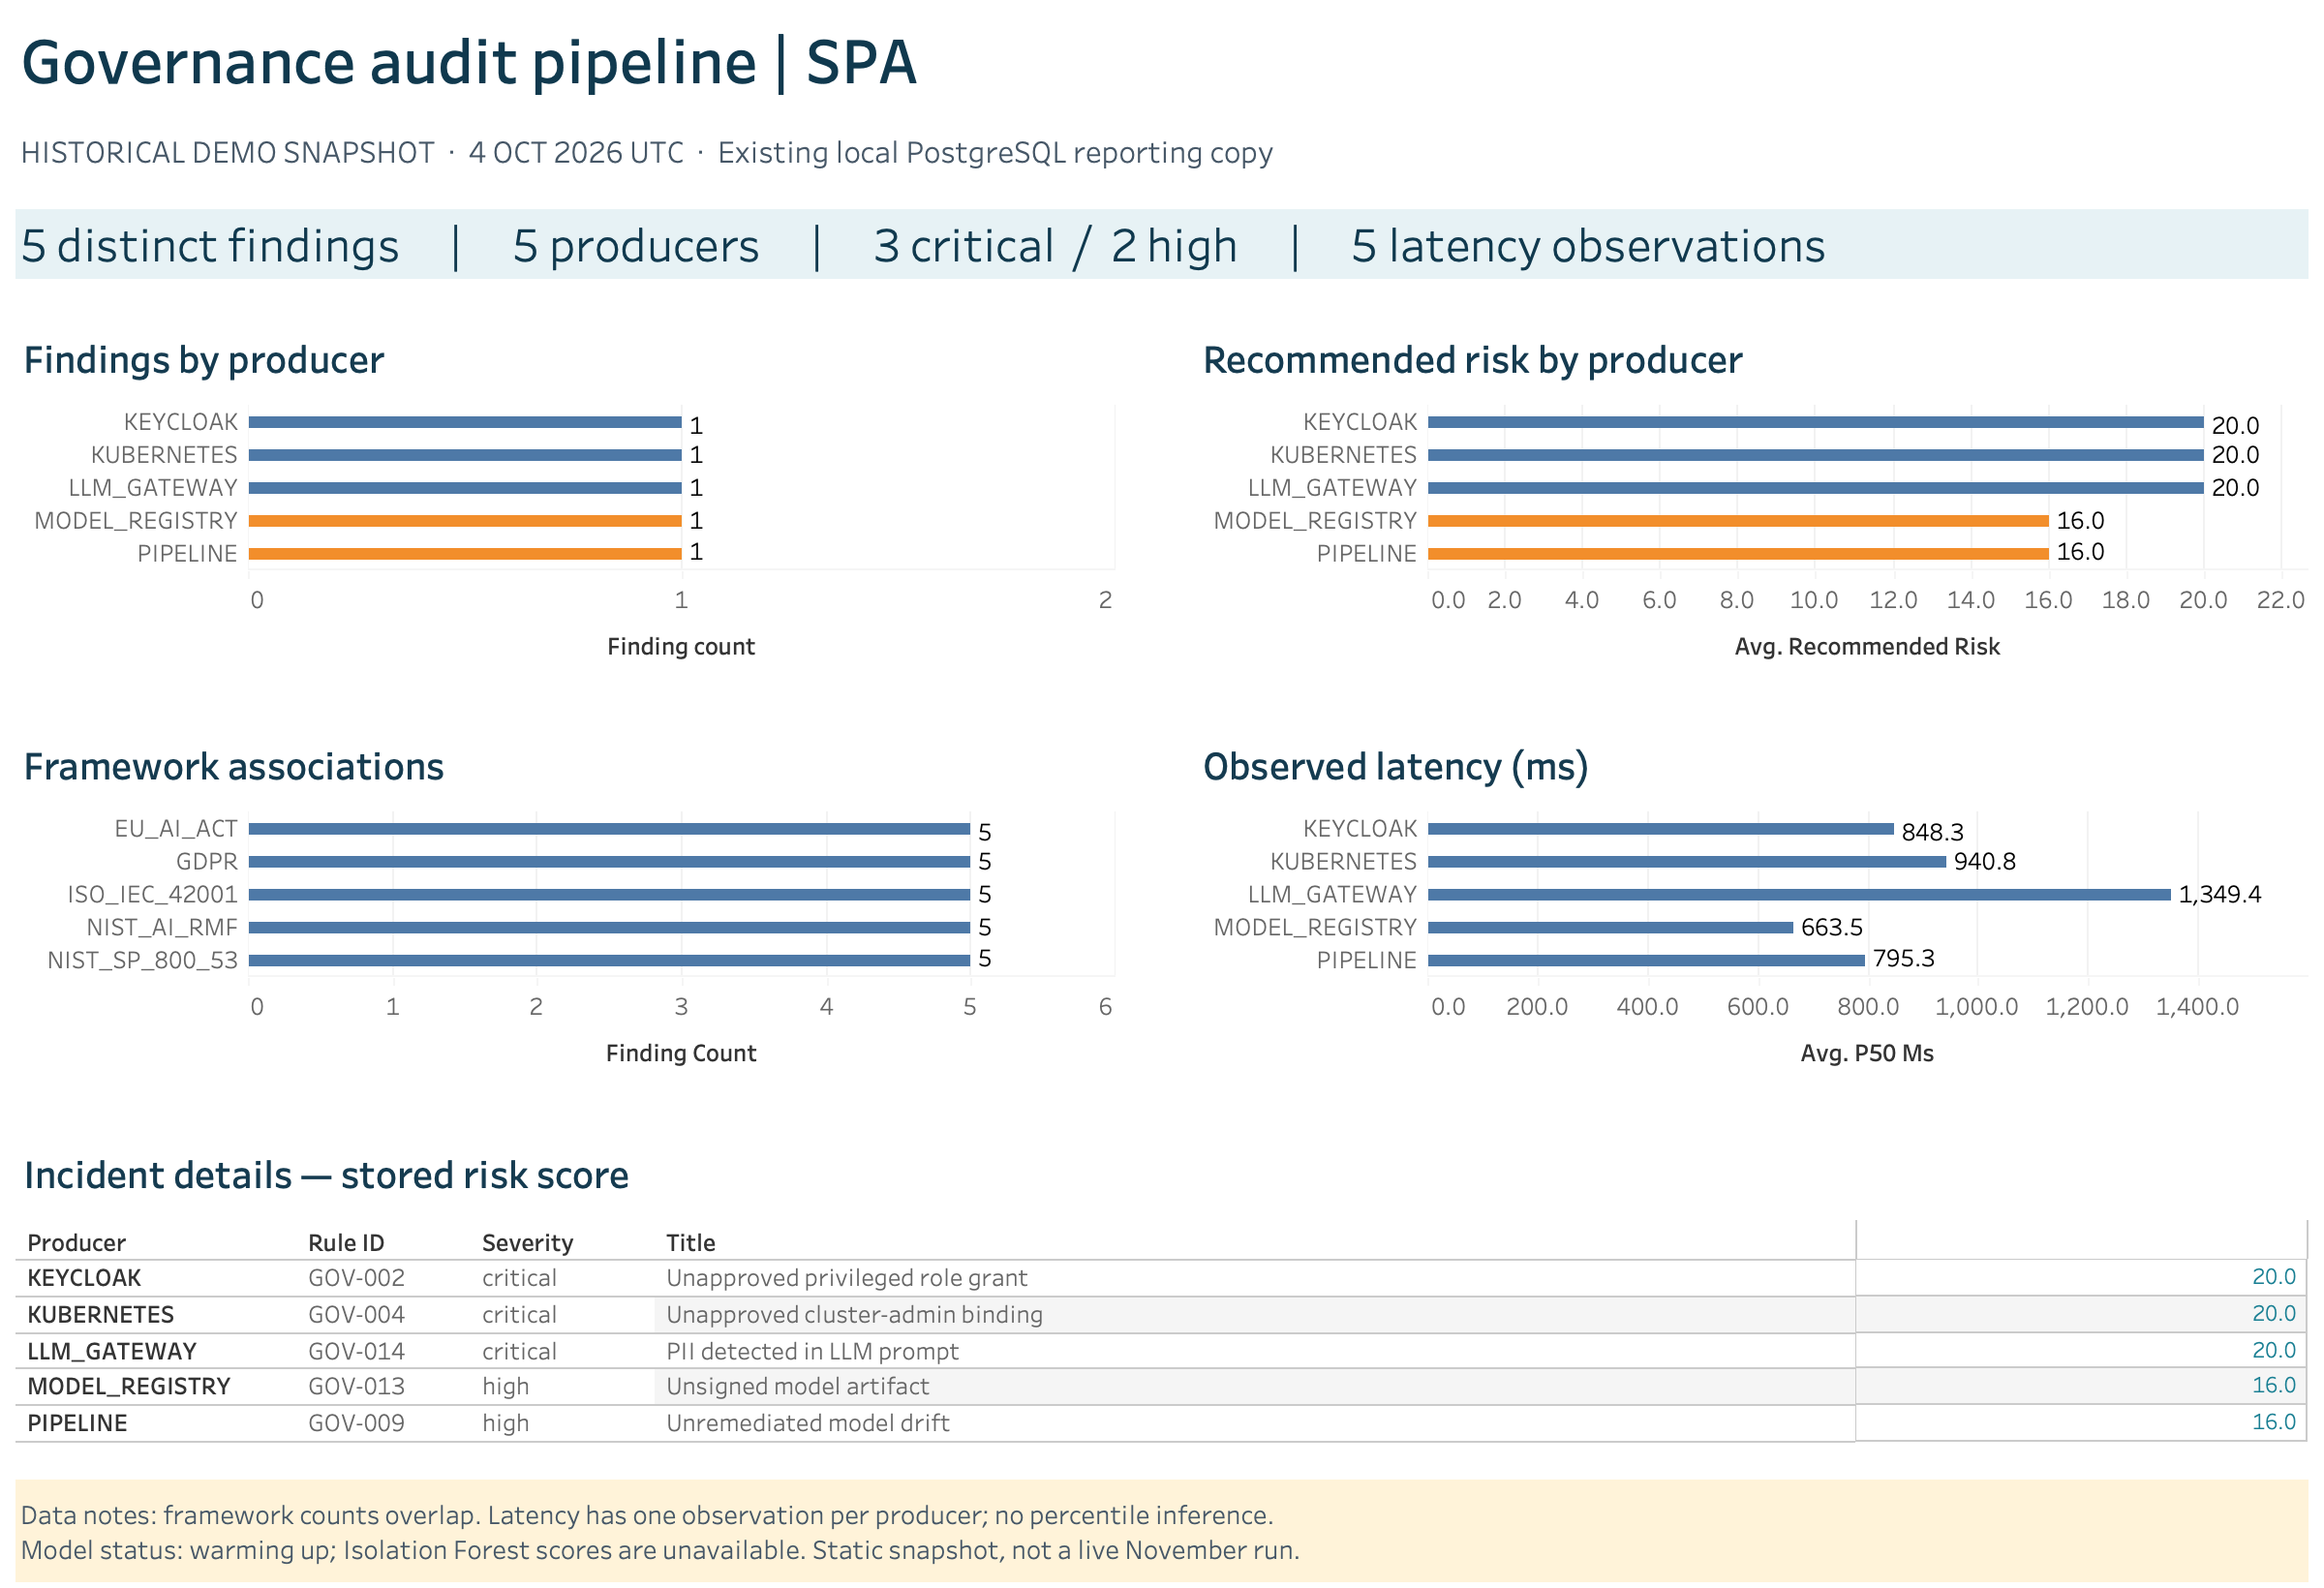
\includegraphics[width=0.92\textwidth,height=0.43\textheight,keepaspectratio]{../report/figures/cloud/09-tableau-dashboard.png}
\caption{Repository-provided Tableau dashboard evidence for the reporting stage.}
\end{figure}

\section*{Traceability summary}
\begin{center}
\begin{tabular}{p{0.25\textwidth}p{0.62\textwidth}}
\toprule
\textbf{Pipeline stage} & \textbf{Source evidence included}\\
\midrule
Producer adapters & Mapper and adapter configuration source\\
Kafka boundary & Docker Compose broker/topic configuration\\
Stream processor & Java Kafka Streams topology\\
Governance controls & YAML rule catalogue\\
Risk and storage & Python scorer and PostgreSQL sink\\
Agent review & Investigator and Reviewer source\\
Evaluation & Results and resilience artefacts\\
Reporting & Tableau reporting schema and dashboard\\
\bottomrule
\end{tabular}
\end{center}

\end{document}
